% --------------------------------------------------------------------------------------------------
% Section: Training
% --------------------------------------------------------------------------------------------------

\section{Training}

% High-level overview of the training strategy, emphasizing fine-tuning of a pre-trained ResNet50.
The training process was designed to fine-tune a pre-trained ResNet50 model for the task of 
multiclass classification (benign, malignant, normal). To ensure efficient and stable learning, 
several key hyperparameters were carefully selected.

% --------------------------------------------------------------------------------------------------
% Subsection: Hyperparameters: Epochs, Learning Rate, Batch Size
% --------------------------------------------------------------------------------------------------

% Subsection discussing the most important hyperparameters used during training.
\subsection{Hyperparameters: Epochs, Learning Rate, Batch Size}

\begin{itemize}
    % Epochs control how many full passes through the training data occur.
    \item \textbf{Epochs:} The training was conducted over \textbf{20 epochs}, meaning the entire 
    dataset was passed through the model ten times. Ten epochs allow the model to learn the 
    underlying patterns without excessive overfitting.

    % Learning rate determines how drastically weights are updated after each batch.
    \item \textbf{Learning rate:} This parameter, a critical one that controls how much the model 
    weights are adjusted during training, was set to \textbf{0.0001}. This low learning rate was 
    chosen to ensure gradual learning, particularly important when fine-tuning a pre-trained 
    network, to avoid overwriting useful features learned from the source dataset.

    % Batch size affects training speed and stability, especially on hardware with limited memory.
    \item \textbf{Batch size:} A \textbf{batch size of 16} was used, which determines the number of 
    samples processed before the model updates its weights. This relatively small batch size was 
    chosen to accommodate CPU-based training and to balance between convergence speed and memory 
    efficiency.
\end{itemize}

\vspace{1em}
\begin{center} 
    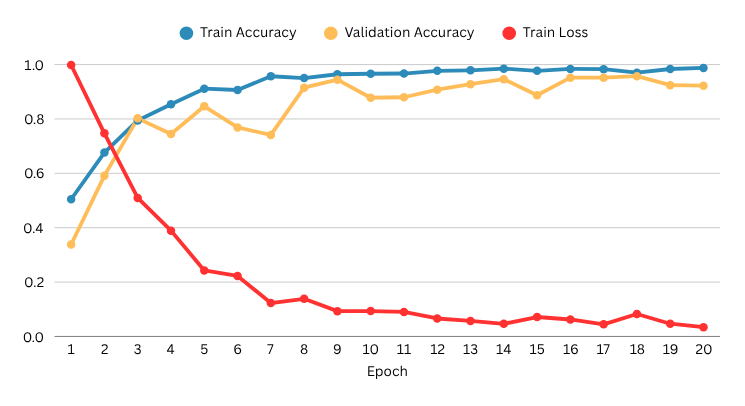
\includegraphics[width=0.7\textwidth]{../assets/05-training/train-evaluation.png} 

    \small\textit{Model training result (accuracy and loss) overview over epochs.}
\end{center}
\vspace{1em}

% --------------------------------------------------------------------------------------------------
% Subsection: Loss Function and Optimizer
% --------------------------------------------------------------------------------------------------

% Subsection explaining the core components that guide how the model learns: the loss function and 
% optimizer.
\subsection{Loss Function and Optimizer}

\begin{itemize}
    % Cross-entropy loss is commonly used for classification tasks involving multiple classes.
    \item \textbf{Loss function:} The loss function used was \textbf{cross-entropy loss}, which is 
    standard for multi-class classification problems. It measures the performance of the 
    classification model by comparing the predicted probabilities to the true class labels, and it 
    encourages the model to assign high probability to the correct class.

    % Mathematical formula for cross-entropy loss displayed below.
    \begin{center}
    \[
    \text{Loss}_{\text{CE}} = - \sum_{i=1}^{C} y_i \log(\hat{y}_i)
    \]
    \end{center}

    % Adam is a widely used optimizer that adjusts learning rates during training.
    \item \textbf{Optimizer:} For optimization, the \textbf{Adam optimizer} was used, which adapts 
    the learning rate for each parameter, combining the advantages of both AdaGrad and RMSProp. 
    This optimizer is particularly well-suited for complex models and noisy gradients, often found 
    in medical image data.
\end{itemize}
